\documentclass[border=4pt]{standalone}
\usepackage{amsmath,tikz}
\usetikzlibrary{braids,arrows.meta,decorations.markings}
\begin{document}
$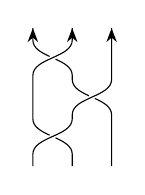
\begin{tikzpicture}[baseline=(current bounding box.center)]
  \pic[draw, yscale=-0.5, braid/width=0.5cm, braid/number of strands=3,
    braid/every strand/.style={postaction={decorate,
      decoration={markings, mark=at position 1 with {\arrow{Stealth[length=5pt]}}}}}]
    (e) {braid={s_1s_2s_1}};
\end{tikzpicture}
\quad = \quad
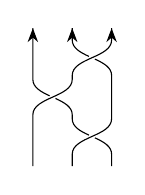
\begin{tikzpicture}[baseline=(current bounding box.center)]
  % Both sides use three strands, as required by the generator s_2.
  \pic[draw, yscale=-0.5, braid/width=0.5cm, braid/number of strands=3,
    braid/every strand/.style={postaction={decorate,
      decoration={markings, mark=at position 1 with {\arrow{Stealth[length=5pt]}}}}}]
    (e) {braid={s_2s_1s_2}};
\end{tikzpicture}$
\end{document}
